\documentclass{standalone}
\usepackage[utf8]{inputenc}
\usepackage[T1]{fontenc}
\usepackage{graphicx}
\usepackage{amsmath}
\usepackage[]{pgf,tikz}
\usepackage[]{circuitikz}
\usetikzlibrary{arrows,shapes,calc,positioning}


\newcommand{\valve}{%
% A clipped circle is drawn
    \draw (0.3,0) arc (0:180:0.3) -- cycle;
    \draw (0,0) -- (0,-0.3);
    \draw (-0.3, -0.15) -- (0.3, -0.45) -- (0.3, -0.15) -- (-0.3, -0.45) -- cycle;
}

\begin{document}
\begin{tikzpicture}
  \footnotesize
  \node (tank1) {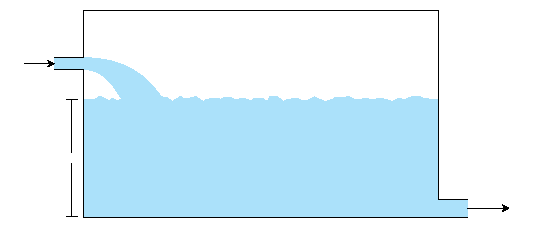
\includegraphics[width=9cm]{tank-with-hole-no-variables}};

\node[] (h1) at (-3.7, -1.5) {$h(t)$};

\node[circle, draw, left of=h1, node distance=1cm, align=center, inner sep=1pt] (LE) {\sf LE\\101};
\node[circle, draw,  left of=LE, node distance=2cm, align=center, inner sep=1pt] (LC) {\sf LC\\101};
\node[coordinate, above of=LC, node distance=26.5mm] (vlv) {};

\coordinate (vlvdraw) at ($(vlv.north) + (0cm, -0.6cm)$);
\coordinate (vlvcontr) at ($(vlv.north) + (0cm, -0.9cm)$);
\coordinate (vlvin) at ($(vlv.west) + (-0.3cm, -0.32cm)$);
\coordinate (vlvout) at ($(vlv.east) + (0.3cm, -0.32cm)$);

\begin{scope}[shift=(vlvdraw), rotate=180] 
  \valve
\end{scope}



\draw[double, thick, double distance=4pt, ] ($(vlvin) - (10mm,0)$) -- (vlvin);
\draw[double, thick, double distance=4pt] (vlvout) -- ($(vlvin) + (3.2,0)$);

\draw (LE) -- ++(4,1.7);
\draw[dashed] (LE) -- (LC);
\draw[dashed] (LC) -- (vlvcontr);

\end{tikzpicture}
\end{document}
